\documentclass[tikz]{standalone}

\usetikzlibrary{decorations.pathmorphing,patterns}

\begin{document}
	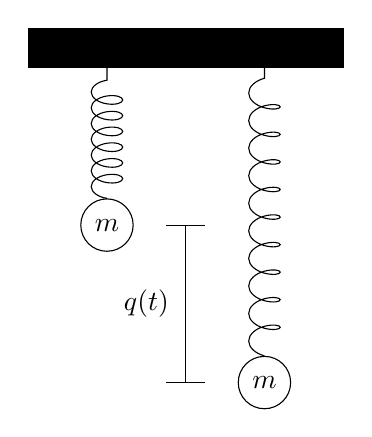
\begin{tikzpicture}
		\node[circle,draw] (m1) at (0,0){$m$};
		\draw[decoration={aspect=0.5, segment length=2mm, amplitude=2mm,coil},decorate] (m1) -- ++(0,2);

		\node[circle,draw] (m2) at (2,-2){$m$};		
		\draw[decoration={aspect=0.5, segment length=3.5mm, amplitude=2mm,coil},decorate] (m2) -- ++(0,4);
		
		\draw[fill=black] (-1,2) rectangle ++(4,0.5);
		
		\draw (m1) ++(0.75,0) -- +(0.5,0);
		\draw (m2) ++(-0.75,0) -- +(-0.5,0);
		\draw (m2) ++(-1,0) -- ++(0,2);
		\node (l) at (0.5,-1){$q(t)$};
	\end{tikzpicture}
\end{document}
